%!TEX root = ../../csuthesis_main.tex
\chapter{研究理论基础}

本章旨在对本研究所依赖的关键算法与基础理论进行系统阐述,为后续视觉目标跟踪与意图识别系统的实现提供理论支撑。内容包括目标检测与视觉跟踪技术的基本概念,DeepSORT 跟踪算法的原理与工作流程,以及基于速度与空间信息的意图识别模型。同时,为便于理解,还将简要介绍在本研究中承担仿真任务的 Carla 平台的相关原理。

\section{目标检测与视觉跟踪概述}

自动驾驶系统当中,环境感知乃是达成安全行驶与智能决策的根基所在,通过计算机视觉技术来识别路上的车辆、行人、交通标志等重要物体,并持续追踪它们的动态状况,这属于完成环境创建以及行为预估的主要方法,目标探测和视觉跟随属于这里面非常关键的形成单元,会径直左右到自动驾驶系统对于周边环境的认识水平及其决策的精准度。

目标检测(Object Detection)即在输入图像当中找出全部存在的感兴趣目标,并精准地对这些目标在图像里的所在位置(一般用边界框来体现)以及所属类别实施回归,传统的目标检测算法大多依靠人工指定的特征加上滑动窗口这种机制,代表性的有Haar特征以及HOG + SVM检测器,此类方法虽然容易做到,但是在面对复杂背景的时候鲁棒性比较差,近些年来,深度学习不断发展起来,依靠卷积神经网络(CNN)的目标检测方法慢慢变成了主流,使得检测的准确率和速度均得到很大改善。 当下主流的检测模型大致可归为两类,其一为以FasterR - CNN作代表的两阶段检测器,该检测器先产生候选区域而后展开类别判断及边框回归操作,此类检测器精度较高,但速度偏慢。另一类是以YOLO(YouOnlyLookOnce),SSD(Single Shot MultiBoxDetector)等为典型的单阶段检测器,它们直接于特征图上实施回归预测,具备更快的即时性,适宜于像自动驾驶这般对时延较为敏感的场合当中。

与目标检测不同,目标跟踪(Object Tracking)是指在已知初始检测结果的前提下,持续对目标在视频序列中的位置进行估计。根据跟踪目标的数量,通常可分为单目标跟踪(Single Object Tracking, SOT)与多目标跟踪(Multiple Object Tracking, MOT)。单目标跟踪关注于对一个特定目标进行持续跟踪,其主要挑战在于遮挡、快速运动、目标消失与再出现等;而多目标跟踪则需要同时对多个目标进行识别与数据关联,面临着更高的关联复杂性与遮挡问题。在实际的自动驾驶场景中,由于交通参与者种类多、状态变化快、相互干扰强,因此往往需在较短时间内完成高准确率的多目标跟踪任务。

视觉目标跟踪往往把目标检测结果当作输入,依靠匹配机制达成目标的跨帧关联,按照是不是利用外部检测结果,跟踪算法可被划列为两类,其中一类是依托检测的跟踪(Tracking - by - Detection),此类方法先通过检测器得到每帧图像里的目标位置,再凭借轨迹预测和数据关联部件来做到目标编号的一致,这属于当下主流的工程化做法;另一类则是端到端的跟踪方法,它直接通过时序特征对目标的运动轨迹执行建模,适宜于复杂行为的建模任务,前面那种因为便于部署而且能和已有检测模型相适应,成了不少自动驾驶感知系统的优先选项。

本研究中,为加强系统的即时性与稳定性,采用“检测-跟踪”分离式结构,也就是先通过图像解析获取候选目标的边界框及状态信息,再借助外部跟踪器(DeepSORT)执行跨帧目标关联,这种结构可兼顾深度检测模型的精准度优势以及目标的运动学特点,达成即时,持续,稳定的目标轨迹追踪,而且还加入了单目标跟踪策略,专门关注当下跟自己车辆存在可能发生交互危险的目标,从而优化后面的意图剖析环节的准确性与实用价值。

目标检测与视觉跟踪技术属于自动驾驶系统感知层的关键支撑部分,会给整个系统的安全,即时以及可靠程度带来直接影响,在这个课题当中,这两项技术处于算法链的起始位置,会给后面的意图识别和行为预测给予基本的信息支持。

\section{DeepSORT 算法原理与流程}

在视觉目标跟踪任务当中,传统的多目标跟踪(MOT)算法诸如SORT(Simple Online and Realtime Tracking),由于其结构较为简单而且处理速度较快,所以被全面地应用到即时系统里面。但是在复杂的交通场景之下,目标相互之间频繁出现遮挡情况,外观相似之处较多,轨迹交叉十分密集等因素,极易引发目标ID发生切换或者导致跟踪过程中断,进而影响到系统的稳定性和实用性,为了解决这些问题,Wojke等人[45]在2017年的时候提出了DeepSORT(Deep Simple Online and Realtime Tracking)算法,该算法在保留SORT轻量级这一特性的前提之下,采用了外观信息来做进一步的数据关联操作,从各个角度加强了多目标跟踪的鲁棒性及其精准度。

\subsection{算法结构概述}

DeepSORT属于依靠检测推动的在线目标追踪算法,它的总体架构包含三个主要部分:目标运动建模单元(卡尔曼滤波器),数据关联单元(匈牙利算法加上结合距离度量)以及外观特征获取单元,它是以SORT(SimpleOnlineandRealtimeTracking)算法为根基加以拓展得来的,SORT算法利用卡尔曼滤波器和匈牙利算法来达成对目标状态的预估以及数据的关联任务,不过仅仅凭借目标的运动信息实施匹配。 DeepSORT通过采用深度学习模型,依靠目标的外观特征进一步提升了算法的鲁棒性和准确性,它的核心思路在于:每一幅图像从检测器那里得到边界框之后,借助预测和匹配把这些边界框同已有的轨迹联系起来,从而做到目标编号的延续以及轨迹的连贯,这样的结构既关注精度又重视即时性,很适宜应用到像自动驾驶这种对时延较为敏感的系统当中。

\subsection{状态预测:卡尔曼滤波器}

DeepSORT 使用卡尔曼滤波器对每个目标进行状态建模与短时位置预测。每个目标的状态向量通常定义为:
\[x = [u, v, \gamma, h, \dot{u}, \dot{v}, \dot{\gamma}, \dot{h}]^{T}\]

DeepSORT的第一步是对目标状态执行预测,这要依靠卡尔曼滤波器来完成,卡尔曼滤波器属于一种凭借动态系统实施状态预估的手段,它可以针对目标的运动状况展开平滑处理并予以预估,这里面牵涉到目标所处的位置,移动速度等等方面,在开展目标追踪的时候,卡尔曼滤波器会遵照前一帧所估算出的目标状态,去推测目标在当前帧大概会处于什么地方,这样就能减小因为目标消失或者被遮挡而产生的误差。

卡尔曼滤波器的核心在于利用目标的运动方程执行线性预估,融合测量值来更新目标的状态,在每一个新的时刻点(即每一帧),它会依照前一帧所得到的目标位置及速度去预测本帧当中目标所处的状态,再通过目标被检测到的实际情况对这一预测加以校正,以此维持目标的连续性,填补检测时可能出现的缺失与错误之处。


\subsection{外观建模:深度特征提取}

在多目标跟踪当中,目标的外观特征获取属于保证算法鲁棒性与精准度的关键技术之列,以往的目标跟踪算法大多依靠目标的运动信息(比如位置,速度之类的)来执行跟踪任务,当遇到目标被遮挡,相互重叠或者高速运动这些情况的时候,通常就难以取得良好的成效。DeepSORT利用深度学习模型,特别就是深度卷积神经网络(CNN),不但可以得到目标的运动信息,而且还能融合其外观特征,从而极大地提升了算法应对复杂场景时的跟踪准确性。

DeepSORT的外观建模部分依靠卷积神经网络(CNN)来获取目标的视觉特征,这些特征往往涵盖目标的颜色,形状,纹理等信息,有益于区分不同目标,特别当多个目标相互重叠或者出现短时被遮挡情况的时候,外观特征可有效地应对身份混淆现象。CNN会针对目标边界框所圈定的区域实施裁剪操作,再把裁剪之后的图像输入到网络当中,从而得到具有固定维度的特征向量,此向量便是目标的外观特征,其体现着目标独有的视觉信息。

通过外观特征获取,DeepSORT可以在跟随时,对比目标于不同帧里的特征向量,以此辨别并区分各个目标,这个办法大幅优化了算法处于复杂动态环境时的性能,特别是当目标相互交错以及被长时间挡住的时候,外观特征给予了一种连续不断的确信度。

不过,外观特征获取不是毫无难题的,在多目标追踪过程中,目标的外观特征也许会被光照,视角改变或者其他环境要素左右,使得目标的视觉特性产生变动,怎样维持特征的一致性,并且在这种变动情况下执行有效的契合,这是DeepSORT碰上的一大难点,对于这个问题,日后的研究能够凭借改良深度网络架构或者融合别的特征获取手段来进一步加强外观建模的稳定性。

总的来说,DeepSORT利用深度学习的外表特征获取机制,让算法不再仅仅依靠目标的运动信息,而且可以凭借视觉特征有效地辨别目标,从而提升了跟踪的准确性和鲁棒性,这项技术对于动态而繁杂场景下的应用有着重大的现实价值,特别适合于自动驾驶,智能监测之类须要精准多目标跟踪的场合。


\subsection{匹配决策:融合距离与匈牙利算法}

在多目标跟踪任务当中,目标的适配决策属于保障跟踪精准度与一致性的关键环节,DeepSORT算法把目标的运动信息和表观特点融合起来实施目标的适配,这样就防止了单纯依靠运动信息而产生的身份混乱和丢失现象,适配决策重点在于通过对目标间相似程度加以计算,并利用改良算法譬如匈牙利算法来执行理想适配。

DeepSORT依靠两种信息去决定目标的契合情况,其一为依托目标位置的欧式距离,其二则是凭借目标外观特征的相似程度,通过这两类信息加以融合之后,DeepSORT就能更为精准地判定当前帧里的检测框同前一帧中的目标是否存在对应关系,确切来讲,欧式距离可用来度量目标在空间中的位置改变状况,至于外观特征方面的相似程度,则体现出目标在视觉空间里所具有的一致性特点。

\textbf{欧氏距离:}多目标跟踪时,目标的位置改变常常体现为目标的运动,欧氏距离是衡量目标在图像空间里位置变化的常见尺度,其计算的是目标在两幅连续图像中的位置差别,目标之间的运动距离越小,表示它们的联系就越密切,于是位置上的距离差异便成了目标契合的关键依照。

\textbf{外观特征的相似度:}为了进一步提升匹配的精准度,DeepSORT会用目标的外观特征做匹配,外观特征通过深度卷积神经网络得到,涵盖目标的颜色,纹理,形状等信息,DeepSORT凭借算出当前帧中目标的外观特征同前一帧里目标特征的相似程度,可以判定两个目标是不是同一个,哪怕它们所处的位置有所改变。

DeepSORT当中,目标的契合决策通过算出每一对目标的契合代价来执行,代价矩阵包含目标间的欧氏距离与外观特征相似度,这两种信息融合成一个全面的契合代价,在此代价矩阵里,每一对目标之间的代价体现出它们相互契合的困难程度,代价越小,表示契合越精准。

DeepSORT要想从代价矩阵当中选出理想的配对,就采用了匈牙利算法,匈牙利算法属于解决二分图匹配难题的典型算法之列,可以在代价矩阵里找出最小的搭配代价,做到目的的理想结合。通过匈牙利算法,DeepSORT就能在当下这一帧和前面那一帧之间寻到最为合适的关联,保障目标身份的连贯性,而且把搭配差错缩减到最少程度。

在实际操作当中,匈牙利算法凭借最优化匹配代价的手段,应对数据关联里目标匹配的状况,把目标检测框同已知目标加以对比,找出最为合适的搭配对子,在复杂的动态环境下,该算法可在目标之间创建起精确的对应联系,缩减目标遗失以及身份错乱现象的发生。

\subsection{算法执行流程}

DeepSORT处理流程包含多个步骤,以下是每帧图像的执行过程:

\textbf{接收当前帧图像和检测器输出(边界框): }在每一帧里面, DeepSORT最先会收到当前帧图像和通过目标探测算法(Yolo,Faster-RCNN等等)所输出的边界框,这些边界框里含有各个目标所处的位置,大小和探测到的可信度。

\textbf{对当前所有轨迹通过卡尔曼滤波器进行状态预测: }DeepSORT针对全部已知目标轨迹,利用卡尔曼滤波器去预估它们的状态,也就是位置与速度,卡尔曼滤波器依照目标在前一帧的位置及速度相关信息,把目标状态加以平滑处理,并对其在当前帧所处的位置予以预测,此步骤有益于填补因为目标丢失或者被遮挡而产生的检测信息空白之处。

\textbf{对当前检测框提取外观特征向量: }DeepSORT利用预先经过训练的深度卷积神经网络(CNN)来获取每一个目标的外观特征,这些外观特征可用来描绘目标的颜色,纹理,形状等视觉方面的信息,依靠这些特征,DeepSORT就能有效地辨别出不一样的目标,即便当目标彼此之间存在遮挡或者其位置发生很大改变的时候,也仍然可以精准地识别并追踪目标。

\textbf{构建融合距离矩阵并输入匈牙利算法匹配轨迹与检测: }DeepSORT依靠目标的运动信息以及外观特征来创建融合距离矩阵,这个矩阵会算出每一个检测框同当前跟踪轨迹之间的匹配程度,其中涵盖了依据位置得出的欧式距离,而且包含了依照外观特征算出的相似系数,之后便利用匈牙利算法针对目标实施最优匹配,以保证每个目标在上一帧和当前帧当中可以精准地关联起来。

\textbf{对匹配成功的轨迹执行更新,未匹配项处理为新轨迹或丢失轨迹: }DeepSORT会更新那些被匹配上的目标的位置,速度之类的信息,而对于没有被匹配上的目标,DeepSORT按照既定的规则来判定到底是把它当成新轨迹也就是新检测到的目标,还是把它当作丢失了的轨迹,丢失的轨迹会依照卡尔曼滤波器所做的预测一直保留着其自身的状态,直至该目标再次出现或者超过了预先指定好的丢失界限值。

\textbf{输出每个有效轨迹的编号与位置: }DeepSORT最后会输出每个有效的目标轨迹,包含目标的编号,位置等信息,各个目标在全部跟踪进程中有个别的ID,以保证目标身份在所有帧里维持一致。

这个流程于每一幅图像当中各自运行,而且可以即时更新目标的状态,所以它有着较好的在线处理能力,非常适宜用在对时延要求比较高的自动驾驶系统,智能监测之类的即时应用场合之中,通过这样一连串的步骤之后,DeepSORT就可以达成对大量目标的精确追踪,即使处于复杂环境之下也能守住较高的即时性能。

\begin{figure}[H]
    \centering
    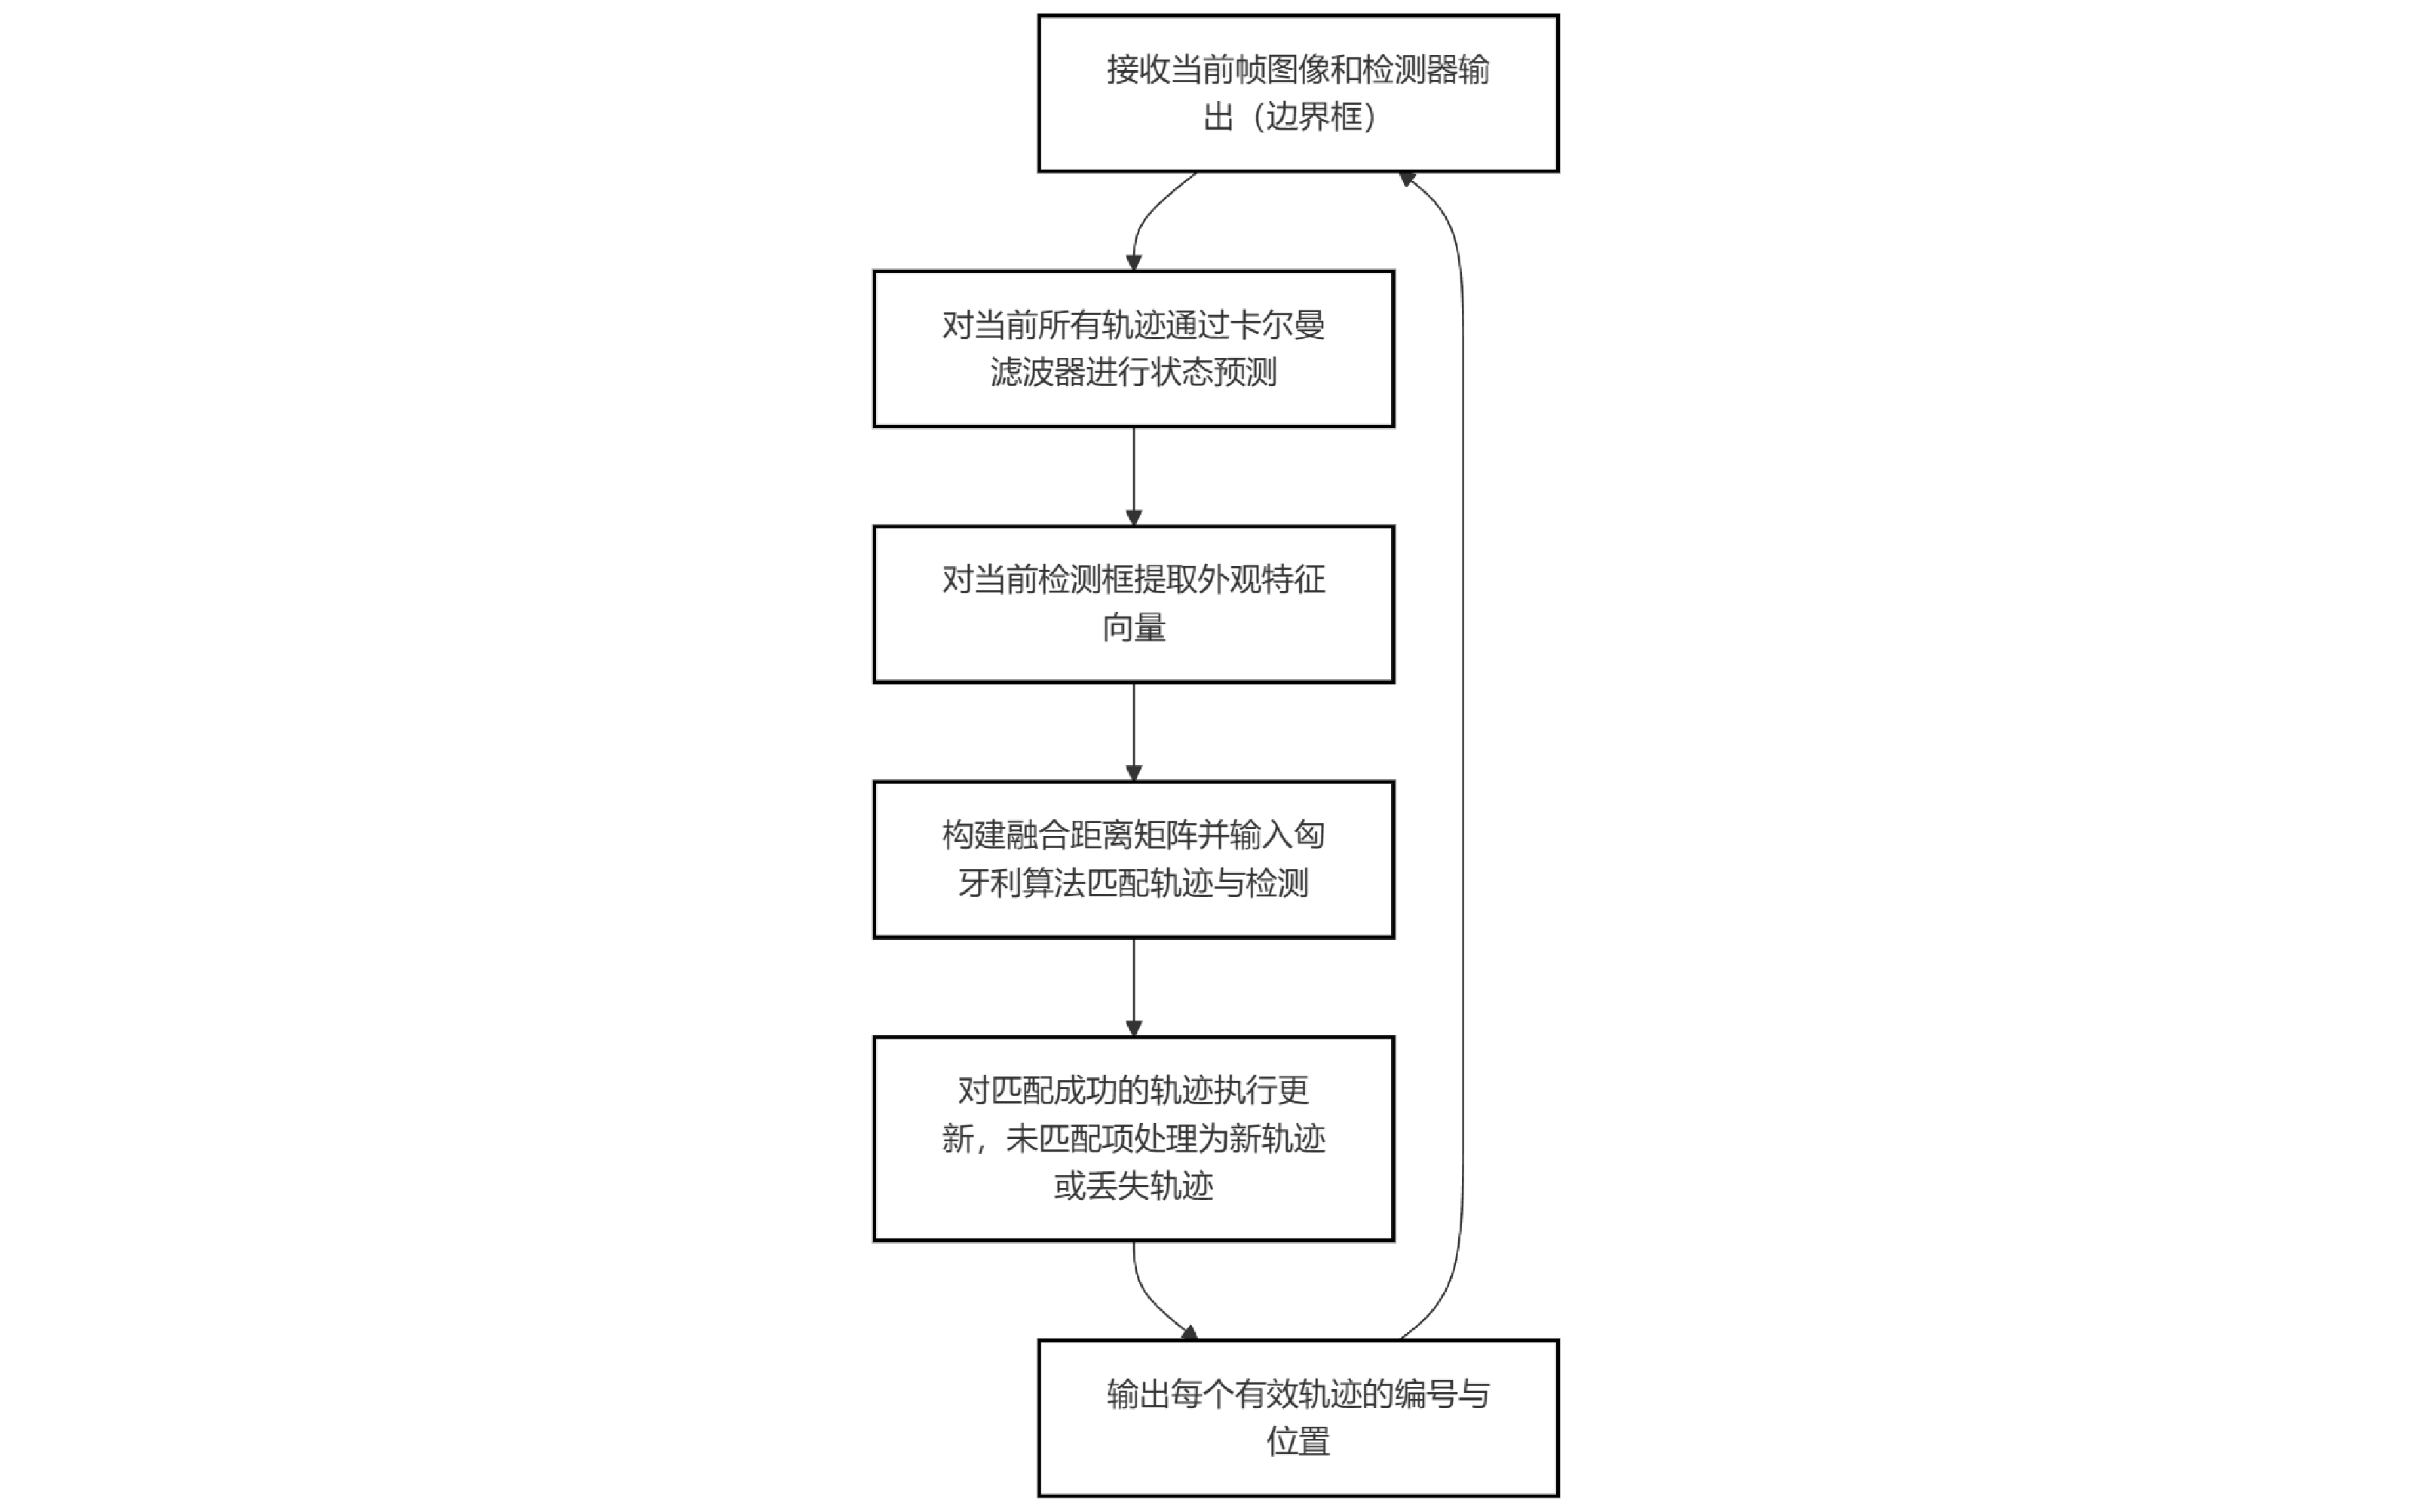
\includegraphics[width=0.8\textwidth]{images/图2 DeepSORT算法执行流程.pdf}  % 引用转换后的 PDF 文件
    \caption{DeepSORT算法执行流程}
    \label{fig:example_image}  % 可用于引用此图片
\end{figure}

\section{行为意图识别的物理建模方法}

自动驾驶系统当中,仅仅具有对环境里物体的“检测”与“跟踪”能力是不够的,想要达成更高层级的决策控制以及路线规划,系统就要去识别周边交通参与者的行为意图,也就是要判定这些参与者日后大概会有怎样的运动趋向,以及他们相对于本车存在何种风险关联,这种行为意图方面的分析既关乎驾驶安全,又同车辆的行为产生策略休戚相关,所以被视作联系感知和决策的重要纽带,在本课题里,对于城市交通环境之下常见的车辆交互情形,规划出一套依靠物理状态信息的行为意图判别手段,并形成起一个能够融入到视觉跟踪体系里的轻型化意图剖析单元。

\subsection{意图识别的物理基础}

本研究所采用的行为意图识别方法,基于目标的相对位置变化与瞬时速度信息,构建了一种近似物理建模的分析机制。设定某一时刻跟踪目标的二维图像平面投影中心($x_t$,$y_t$),上一时刻为($x_{t-1}$,$y_{t-1}$),自车屏幕参考点位置为($x_c$,$y_c$)。则目标相对位置变化量可定义为:
\[\Delta d = \|(x_t, y_t) - (x_c, y_c)\| - \|(x_{t - 1}, y_{t - 1}) - (x_c, y_c)\|\]

其中,$\left| \cdot \right|$表示欧几里得距离。该值用于衡量目标与自车的相对距离变化趋势。结合目标的瞬时速度$v_t$,可初步判断其运动意图。

此外,为增强分析的动态敏感性,引入了前后帧距离差分值$\Delta d$与速度 $v_t$的联合判断阈值规则。通过组合判断目标是否正在靠近本车、远离、停留或加速穿越等,从而实现意图的粗分类。这种方法不依赖于轨迹预测或时序模型,具有实现简单、计算开销小、适用于实时系统等优点。

\subsection{判别规则设计与分类逻辑}

在本研究系统中,结合实验场景和工程实现,设计了以下几种典型的行为状态分类逻辑:

\textbf{目标靠近中:}当$\Delta d < -\delta_{\mathrm{d}}$且$v_t>v_{\text{min}}$时,表明目标正在快速靠近自车;

\textbf{目标远离中:}当$\Delta d > -\delta_{\mathrm{d}}$时,目标正在逐渐离开;

\textbf{危险靠近:}若当前距离低于设定阈值$d_{\text{critical}}$且速度超过$v_{\text{danger}}$时,则标记为潜在危险行为;

\textbf{目标稳定:}若目标距离变化缓慢或速度较低,判断为意图不明或保持状态;

\textbf{目标初始化中:}用于系统首次观测目标,未形成完整判断所处状态。

上述分类逻辑采用了硬阈值判定策略,其参数$\delta_{\mathrm{d}}$、$v_{\text{min}}$、$v_{\text{danger}}$、$d_{\text{critical}}$均可根据场景密度或车辆速度进行调节。在实验中,采用经验法则设定$\delta_{\mathrm{d}}$=5、$v_{\text{min}}$=1.5m/s、$v_{\text{danger}}$=3.0m/s、$d_{\text{critical}}$=150(像素),实现了较高的判别正确率。

\subsection{与视觉跟踪系统的集成实现}

本意图分析模块在执行时嵌于单目标跟踪模块之后,它会针对被选中目标的时序状态展开分析,输出当前帧的意图状态表述文本,而且会在图像上即时显现出来,该模块还规划了状态缓存机制,以保障判断结果具有一定的时间连贯性,免除由于短时检测偏差造成意图颤抖现象发生。

在Carla仿真平台的Town10与Town01场景当中,这个模块达成了对于前方车辆是否出现“威胁靠近”或者“远离离散”情况的视觉提示效果,从而加强了整个系统的交互解释性以及安全回应能力,给后续的路线规划和驾驶行为产生赋予了语义层面的输入支撑。

\section{小结}

这一章着眼于“视觉目标追踪和行为意图识别”在自动驾驶系统里的主要功能,详细论述了此课题研究依靠的有关理论和重要技术,第一,考虑到当下智能驾驶车辆对于处在动态环境时感知能力的优化需求,简单总结了目标检测和视觉追踪的发展过程,剖析了从依靠运动模型的传统追踪手段,到结合检测器成果和深度特性的当代方法所经历的技术改进,通过整理视觉感知的整个流程,清楚表明了视觉追踪在动态交通场景下对目标连贯性,身份维持以及行为判定起到的无法被取代的意义。

其次,论文着重剖析了本研究里用到的DeepSORT算法的主要原理及其完整处理流程,这个算法既保留了传统SORT算法速度方面的长处,又加入了外观特征建模机制,从而较好地解决了目标被遮挡,遮蔽之后re - identification(再识别)失败之类的问题。论文针对DeepSORT当中的卡尔曼滤波器状态建模,ReID特征获取网络,把马氏距离和余弦距离相融合的度量机制,还有轨迹适配及更新策略做了逐个解读,而且阐述了此算法在本系统中的实际操作情况,也就是怎样联系检测成果来达成在线目标轨迹的更新,进而输出稳定且可控制的目标标识编号,给后面的高层语义分析形成根基。

第三部分当中,这一章也详细探究了行为意图识别的物理建模办法,相比依靠深度学习的预测模型或者时序模型,此项研究采取更为轻巧,高效并且适合于即时场景的依靠位置与速度信息的规则建模策略,这个方法把相对距离的改变和目标的运动速度联系起来形成一种复合条件的判别机制,这样就能识别出诸如“靠近”“远离”“危险逼近”这些具有代表性的语义意图。该模块在执行方面被合并到目标追踪逻辑后面,通过接连帧的数据开展物理量运算并配合阈值策略来达成对于动态交互行为的解读与警示,而且,为了改善系统的互动性和直接表现效果,本研究创建了相应的视觉化机制,会把判别结果立刻添加到目标标识框之上,进一步优化了系统针对繁杂交通行为的回应水平及解读水平。

综合而言,这一章站在理论层面上,全面整理了本课题里有关视觉感知,目标追踪以及行为认知这些重要部分,给后面整个系统功能的达成形成稳固的技术根基,下一章会依靠这一章的理论铺垫,细致地阐述系统总体架构的设计想法,包含Carla仿真平台怎样设置,自动驾驶控制主要模块如何创建,还有整体工程开发环境怎样营造等方面,从工程方面来促使本研究方案得以落实。


\begin{tabular}{l l}
%  \verb|\songti| & {\songti 宋体} \\
%  \verb|\heiti| & {\heiti 黑体} \\
%   \verb|\kaiti| & {\kaiti 楷体}
\end{tabular}
